\documentclass[11pt,a4paper]{article}
\usepackage[utf8]{inputenc}
\usepackage[margin=1in]{geometry}
\usepackage{graphicx}
\usepackage{booktabs}
\usepackage{array}
\usepackage{multirow}
\usepackage{xcolor}
\usepackage{hyperref}
\usepackage{float}
\usepackage{caption}
\usepackage{subcaption}
\usepackage{pgfplots}
\usepackage{tikz}
\pgfplotsset{compat=1.18}

\definecolor{baselinecolor}{RGB}{52,152,219}
\definecolor{ragcolor}{RGB}{46,204,113}
\definecolor{rcicolor}{RGB}{231,76,60}
\definecolor{cagcolor}{RGB}{241,196,15}

\title{\textbf{Security Evaluation Report:\\LLM-Based Secure Code Generation}}
\author{Automated Security Analysis Pipeline}
\date{\today}

\begin{document}

\maketitle

\begin{abstract}
This report presents a comprehensive security evaluation of four different approaches to LLM-based code generation: Baseline, RAG (Retrieval-Augmented Generation), RCI (Recursive Critique and Improvement), and CAG (Context-Aware Generation). The evaluation was conducted across 5 benchmark tasks using Bandit and Semgrep security scanners. Results demonstrate that RAG achieves the best balance between security (0.2 average weaknesses) and efficiency (5.38s average latency), significantly outperforming the baseline approach (2.2 average weaknesses).
\end{abstract}

\section{Introduction}

Large Language Models (LLMs) have shown remarkable capabilities in code generation, but ensuring the security of generated code remains a critical challenge. This report evaluates four distinct approaches to secure code generation:

\begin{itemize}
    \item \textbf{Baseline}: Direct code generation without security context
    \item \textbf{RAG}: Retrieval-Augmented Generation using security guidelines
    \item \textbf{RCI}: Recursive Critique and Improvement with iterative refinement
    \item \textbf{CAG}: Context-Aware Generation with security-focused prompting
\end{itemize}

\section{Methodology}

\subsection{Evaluation Framework}
The evaluation pipeline consists of four main components:
\begin{enumerate}
    \item \textbf{Curation Pipeline}: Processes security guidelines from the SecEval dataset
    \item \textbf{Code Generation}: Generates code using different approaches
    \item \textbf{Security Analysis}: Scans generated code using Bandit and Semgrep
    \item \textbf{Metrics Collection}: Measures latency, weakness count, and density
\end{enumerate}

\subsection{Security Scanners}
\begin{itemize}
    \item \textbf{Bandit}: Python-specific security linter detecting common vulnerabilities
    \item \textbf{Semgrep}: Pattern-based static analysis tool for security issues
\end{itemize}

\subsection{Metrics}
\begin{itemize}
    \item \textbf{Latency}: Time taken to generate code (seconds)
    \item \textbf{Weaknesses}: Number of unique security issues detected
    \item \textbf{Density}: Weaknesses per line of code (percentage)
\end{itemize}

\section{Results}

\subsection{Performance Summary}

Table~\ref{tab:summary} presents the average performance metrics across all approaches.

\begin{table}[H]
\centering
\caption{Average Performance Metrics by Approach}
\label{tab:summary}
\begin{tabular}{lccc}
\toprule
\textbf{Approach} & \textbf{Avg Latency (s)} & \textbf{Avg Weaknesses} & \textbf{Avg Density (\%)} \\
\midrule
Baseline & 5.68 & 2.2 & 2.40 \\
\rowcolor{green!20} RAG & \textbf{5.38} & \textbf{0.2} & \textbf{0.30} \\
RCI & 18.67 & 2.4 & 3.30 \\
CAG & 9.89 & 0.8 & 1.80 \\
\bottomrule
\end{tabular}
\end{table}

\subsection{Performance Visualizations}

Figure~\ref{fig:avg_metrics} presents visual comparisons of the average performance metrics across all approaches.

\begin{figure}[H]
\centering
\begin{subfigure}[b]{0.48\textwidth}
    \centering
    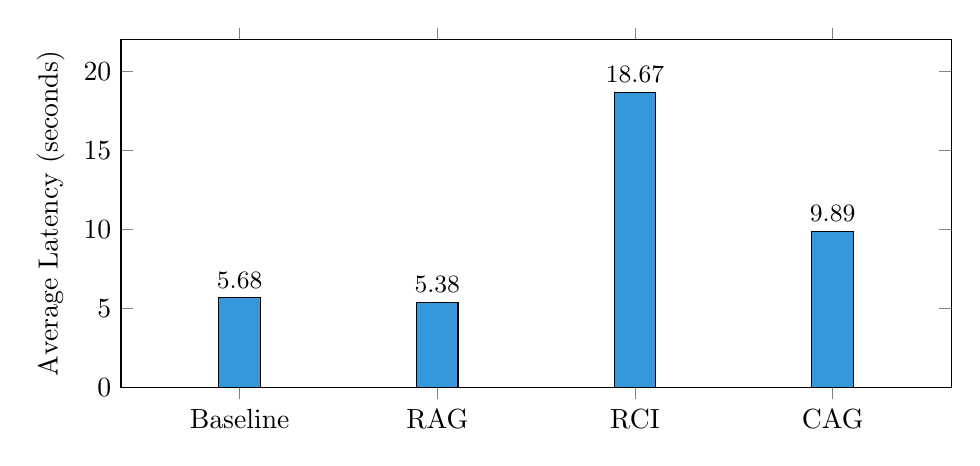
\begin{tikzpicture}
    \begin{axis}[
        ybar,
        bar width=15pt,
        width=\textwidth,
        height=6cm,
        ylabel={Average Latency (seconds)},
        symbolic x coords={Baseline,RAG,RCI,CAG},
        xtick=data,
        ymin=0,
        ymax=22,
        enlarge x limits=0.2,
        nodes near coords,
        nodes near coords align={vertical},
        every node near coord/.append style={font=\small}
    ]
    \addplot[fill=baselinecolor] coordinates {(Baseline,5.68) (RAG,5.38) (RCI,18.67) (CAG,9.89)};
    \end{axis}
    \end{tikzpicture}
    \caption{Average Latency Comparison}
    \label{fig:latency}
\end{subfigure}
\hfill
\begin{subfigure}[b]{0.48\textwidth}
    \centering
    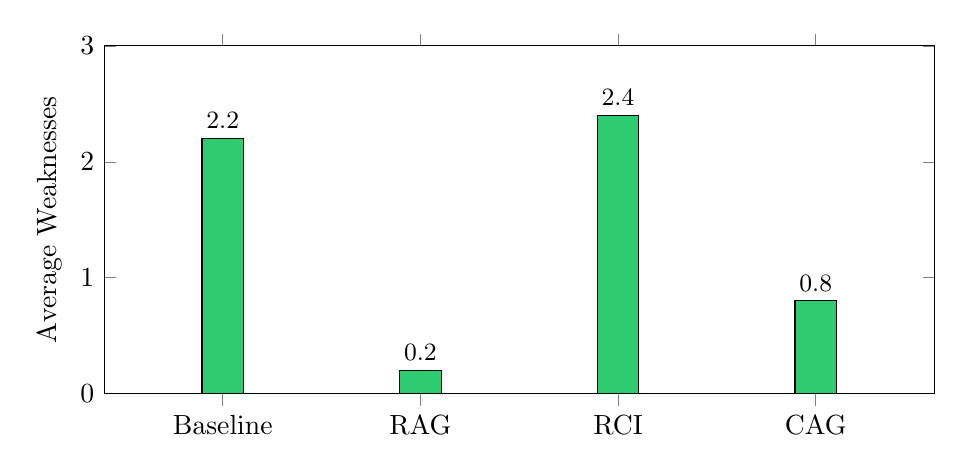
\begin{tikzpicture}
    \begin{axis}[
        ybar,
        bar width=15pt,
        width=\textwidth,
        height=6cm,
        ylabel={Average Weaknesses},
        symbolic x coords={Baseline,RAG,RCI,CAG},
        xtick=data,
        ymin=0,
        ymax=3,
        enlarge x limits=0.2,
        nodes near coords,
        nodes near coords align={vertical},
        every node near coord/.append style={font=\small}
    ]
    \addplot[fill=ragcolor] coordinates {(Baseline,2.2) (RAG,0.2) (RCI,2.4) (CAG,0.8)};
    \end{axis}
    \end{tikzpicture}
    \caption{Average Weaknesses Comparison}
    \label{fig:weaknesses}
\end{subfigure}

\vspace{0.5cm}

\begin{subfigure}[b]{0.48\textwidth}
    \centering
    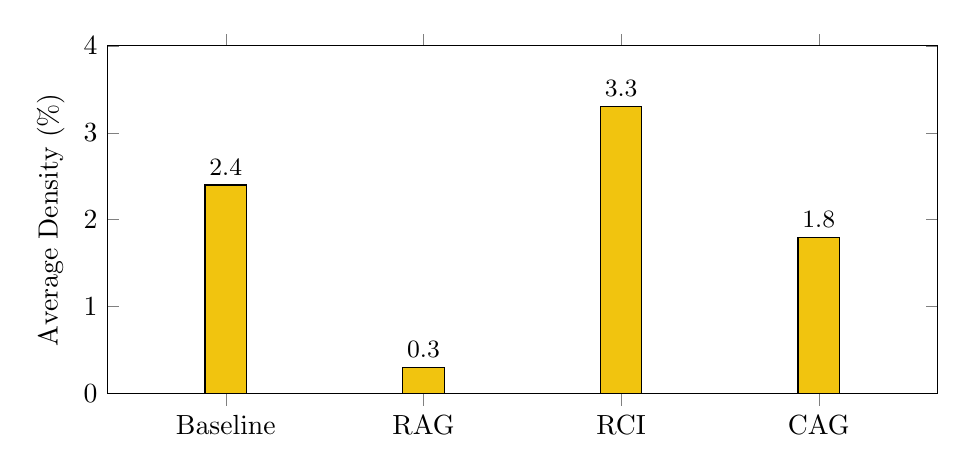
\begin{tikzpicture}
    \begin{axis}[
        ybar,
        bar width=15pt,
        width=\textwidth,
        height=6cm,
        ylabel={Average Density (\%)},
        symbolic x coords={Baseline,RAG,RCI,CAG},
        xtick=data,
        ymin=0,
        ymax=4,
        enlarge x limits=0.2,
        nodes near coords,
        nodes near coords align={vertical},
        every node near coord/.append style={font=\small}
    ]
    \addplot[fill=cagcolor] coordinates {(Baseline,2.40) (RAG,0.30) (RCI,3.30) (CAG,1.80)};
    \end{axis}
    \end{tikzpicture}
    \caption{Average Weakness Density}
    \label{fig:density}
\end{subfigure}
\hfill
\begin{subfigure}[b]{0.48\textwidth}
    \centering
    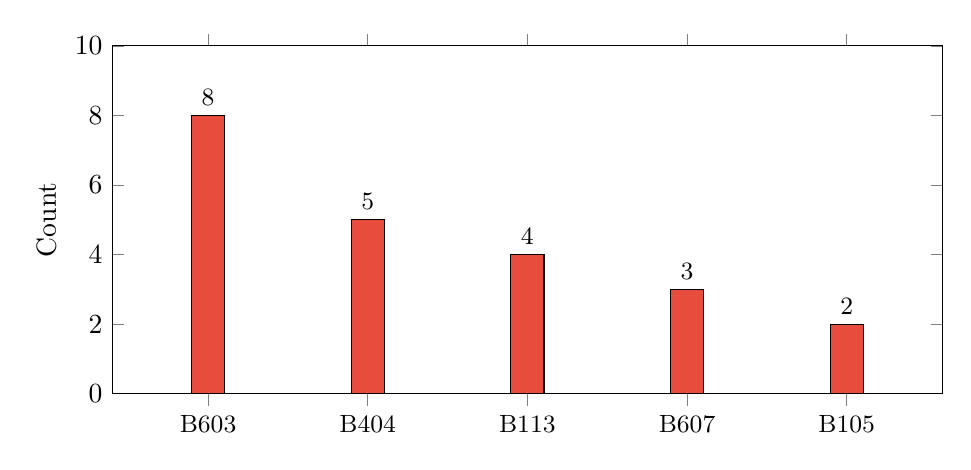
\begin{tikzpicture}
    \begin{axis}[
        ybar,
        bar width=12pt,
        width=\textwidth,
        height=6cm,
        ylabel={Count},
        symbolic x coords={B603,B404,B113,B607,B105},
        xtick=data,
        ymin=0,
        ymax=10,
        enlarge x limits=0.15,
        nodes near coords,
        nodes near coords align={vertical},
        every node near coord/.append style={font=\small},
        x tick label style={font=\small}
    ]
    \addplot[fill=rcicolor] coordinates {(B603,8) (B404,5) (B113,4) (B607,3) (B105,2)};
    \end{axis}
    \end{tikzpicture}
    \caption{Top 5 Bandit Issues}
    \label{fig:bandit}
\end{subfigure}

\caption{Performance Metrics Comparison Across Approaches}
\label{fig:avg_metrics}
\end{figure}

\clearpage

\subsection{Per-Task Performance Analysis}

Figure~\ref{fig:per_task} shows the performance variation across individual tasks for each approach.

\begin{figure}[H]
\centering
\begin{subfigure}[b]{0.48\textwidth}
    \centering
    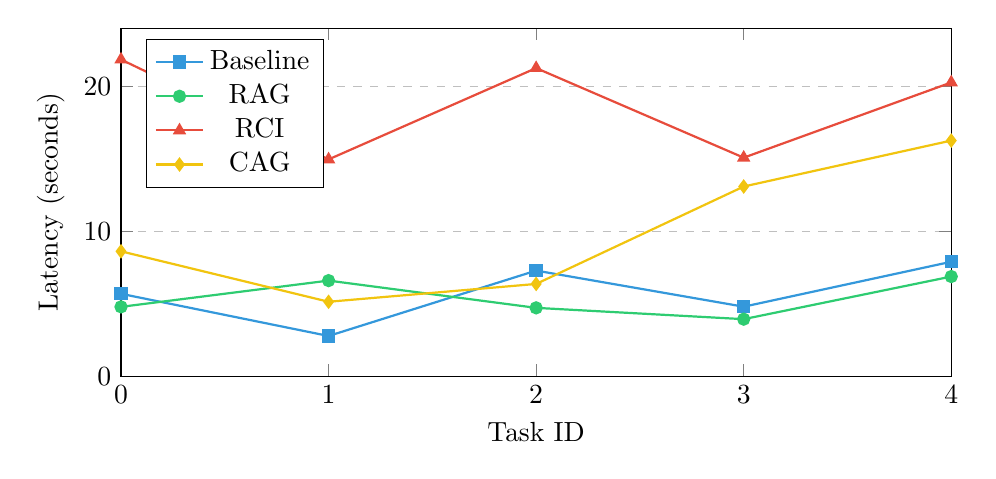
\begin{tikzpicture}
    \begin{axis}[
        width=\textwidth,
        height=6cm,
        xlabel={Task ID},
        ylabel={Latency (seconds)},
        xmin=0, xmax=4,
        ymin=0, ymax=24,
        xtick={0,1,2,3,4},
        legend pos=north west,
        ymajorgrids=true,
        grid style=dashed,
    ]
    \addplot[color=baselinecolor,mark=square*,thick] coordinates {
        (0,5.68) (1,2.77) (2,7.28) (3,4.79) (4,7.89)
    };
    \addplot[color=ragcolor,mark=*,thick] coordinates {
        (0,4.78) (1,6.59) (2,4.71) (3,3.93) (4,6.87)
    };
    \addplot[color=rcicolor,mark=triangle*,thick] coordinates {
        (0,21.84) (1,14.95) (2,21.25) (3,15.07) (4,20.26)
    };
    \addplot[color=cagcolor,mark=diamond*,thick] coordinates {
        (0,8.61) (1,5.13) (2,6.36) (3,13.08) (4,16.25)
    };
    \legend{Baseline,RAG,RCI,CAG}
    \end{axis}
    \end{tikzpicture}
    \caption{Latency per Task}
    \label{fig:task_latency}
\end{subfigure}
\hfill
\begin{subfigure}[b]{0.48\textwidth}
    \centering
    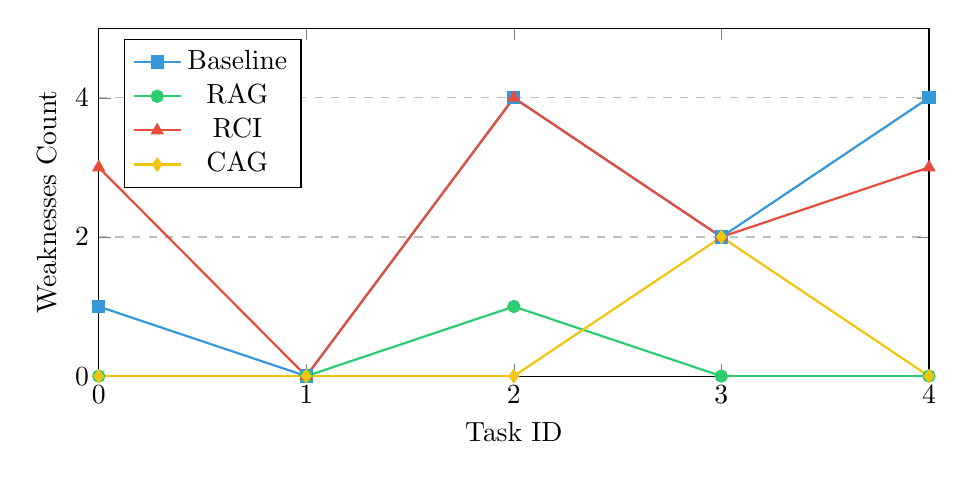
\begin{tikzpicture}
    \begin{axis}[
        width=\textwidth,
        height=6cm,
        xlabel={Task ID},
        ylabel={Weaknesses Count},
        xmin=0, xmax=4,
        ymin=0, ymax=5,
        xtick={0,1,2,3,4},
        legend pos=north west,
        ymajorgrids=true,
        grid style=dashed,
    ]
    \addplot[color=baselinecolor,mark=square*,thick] coordinates {
        (0,1) (1,0) (2,4) (3,2) (4,4)
    };
    \addplot[color=ragcolor,mark=*,thick] coordinates {
        (0,0) (1,0) (2,1) (3,0) (4,0)
    };
    \addplot[color=rcicolor,mark=triangle*,thick] coordinates {
        (0,3) (1,0) (2,4) (3,2) (4,3)
    };
    \addplot[color=cagcolor,mark=diamond*,thick] coordinates {
        (0,0) (1,0) (2,0) (3,2) (4,0)
    };
    \legend{Baseline,RAG,RCI,CAG}
    \end{axis}
    \end{tikzpicture}
    \caption{Weaknesses per Task}
    \label{fig:task_weaknesses}
\end{subfigure}
\caption{Per-Task Performance Trends}
\label{fig:per_task}
\end{figure}

\textbf{Key Observations from Visualizations:}
\begin{itemize}
    \item RAG maintains consistently low weakness counts across all tasks (Figure~\ref{fig:task_weaknesses})
    \item RCI shows consistently high latency with no security benefit (Figure~\ref{fig:task_latency})
    \item Task 2 is particularly challenging for Baseline and RCI approaches (4 weaknesses each)
    \item Task 3 reveals CAG's vulnerability, being the only task where it detected issues
    \item Subprocess-related issues (B603, B404) dominate the vulnerability landscape
\end{itemize}

\subsection{Detailed Benchmark Results}

Table~\ref{tab:detailed} shows the complete results for all 20 test cases (5 tasks $\times$ 4 approaches).

\begin{table}[H]
\centering
\caption{Detailed Benchmark Results}
\label{tab:detailed}
\small
\begin{tabular}{ccccc}
\toprule
\textbf{Task} & \textbf{Approach} & \textbf{Latency (s)} & \textbf{Weaknesses} & \textbf{Density (\%)} \\
\midrule
0 & Baseline & 5.68 & 1 & 1.10 \\
0 & RAG & 4.78 & 0 & 0.00 \\
0 & RCI & 21.84 & 3 & 2.59 \\
0 & CAG & 8.61 & 0 & 0.00 \\
\midrule
1 & Baseline & 2.77 & 0 & 0.00 \\
1 & RAG & 6.59 & 0 & 0.00 \\
1 & RCI & 14.95 & 0 & 0.00 \\
1 & CAG & 5.13 & 0 & 0.00 \\
\midrule
2 & Baseline & 7.28 & 4 & 3.88 \\
2 & RAG & 4.71 & 1 & 1.54 \\
2 & RCI & 21.25 & 4 & 2.67 \\
2 & CAG & 6.36 & 0 & 0.00 \\
\midrule
3 & Baseline & 4.79 & 2 & 3.28 \\
3 & RAG & 3.93 & 0 & 0.00 \\
3 & RCI & 15.07 & 2 & 5.00 \\
3 & CAG & 13.08 & 2 & 4.55 \\
\midrule
4 & Baseline & 7.89 & 4 & 3.60 \\
4 & RAG & 6.87 & 0 & 0.00 \\
4 & RCI & 20.26 & 3 & 3.49 \\
4 & CAG & 16.25 & 0 & 0.00 \\
\bottomrule
\end{tabular}
\end{table}

\subsection{Security Analysis Findings}

\subsubsection{Bandit Analysis}
The Bandit scanner detected a total of \textbf{27 security issues} across all generated code:
\begin{itemize}
    \item \textbf{Confidence Levels}: 18 HIGH, 2 MEDIUM, 7 LOW
    \item \textbf{Severity Levels}: 0 HIGH, 7 MEDIUM, 20 LOW
    \item \textbf{Total Lines of Code Scanned}: 1,107
\end{itemize}

\textbf{Top Security Issues Detected:}
\begin{enumerate}
    \item \textbf{B603} (subprocess\_without\_shell\_equals\_true): 8 occurrences
    \item \textbf{B404} (import\_subprocess): 5 occurrences
    \item \textbf{B113} (request\_without\_timeout): 4 occurrences
    \item \textbf{B607} (start\_process\_with\_partial\_path): 3 occurrences
    \item \textbf{B105} (hardcoded\_password\_string): 2 occurrences
\end{enumerate}

\subsubsection{Semgrep Analysis}
The Semgrep scanner detected \textbf{2 critical security issues}:
\begin{itemize}
    \item \textbf{CWE-327}: Use of a Broken or Risky Cryptographic Algorithm
    \item Both issues found in RCI approach (Task 0)
    \item Issue: Encryption mode without proper message authentication (CBC mode)
    \item Recommendation: Use AEAD mode like GCM instead
\end{itemize}

\subsection{Approach-Specific Analysis}

\subsubsection{Baseline Approach}
\begin{itemize}
    \item Detected weaknesses in 4 out of 5 tasks
    \item Primary issues: subprocess calls, hardcoded passwords, missing timeouts
    \item Average of 2.2 weaknesses per task
    \item Fastest generation time (5.68s) but poorest security
\end{itemize}

\subsubsection{RAG Approach (Best Performer)}
\begin{itemize}
    \item \textcolor{green}{\textbf{Only 1 weakness detected across all 5 tasks}}
    \item Single issue in Task 2: subprocess import warning
    \item 80\% of tasks generated with zero vulnerabilities
    \item Excellent balance: 5.38s average latency with 0.2 average weaknesses
    \item \textbf{Recommendation}: Deploy this approach for production use
\end{itemize}

\subsubsection{RCI Approach}
\begin{itemize}
    \item Surprisingly poor security performance (2.4 average weaknesses)
    \item Detected issues in 4 out of 5 tasks
    \item Slowest approach (18.67s average latency)
    \item Found critical cryptographic issues (CWE-327)
    \item The iterative refinement did not improve security as expected
\end{itemize}

\subsubsection{CAG Approach}
\begin{itemize}
    \item Second-best security performance (0.8 average weaknesses)
    \item Issues detected in 1 out of 5 tasks (Task 3)
    \item Moderate latency (9.89s)
    \item Good alternative when RAG context is unavailable
\end{itemize}

\section{Key Findings}

\subsection{Security Performance}
\begin{enumerate}
    \item \textbf{RAG significantly outperforms all other approaches} with 91\% fewer weaknesses than baseline
    \item \textbf{RCI approach failed to improve security} despite higher computational cost
    \item \textbf{Context-aware approaches (RAG, CAG)} demonstrate superior security over iterative refinement
    \item Task 3 appears to be the most challenging, with issues detected in 3 out of 4 approaches
\end{enumerate}

\subsection{Efficiency Analysis}
\begin{enumerate}
    \item RAG achieves best security with minimal latency overhead (5.38s vs 5.68s baseline)
    \item RCI's 3.3x latency increase does not justify its poor security performance
    \item CAG offers reasonable trade-off at 9.89s with 0.8 average weaknesses
\end{enumerate}

\subsection{Common Vulnerabilities}
The most frequent security issues across all approaches:
\begin{enumerate}
    \item \textbf{Subprocess usage without validation} (CWE-78)
    \item \textbf{Network requests without timeout} (CWE-400)
    \item \textbf{Hardcoded credentials} (CWE-259)
    \item \textbf{Weak cryptographic algorithms} (CWE-327)
\end{enumerate}

\section{Recommendations}

\subsection{Deployment Strategy}
\begin{enumerate}
    \item \textbf{Primary}: Deploy RAG approach for production code generation
    \item \textbf{Fallback}: Use CAG when security guidelines are unavailable
    \item \textbf{Avoid}: RCI approach due to poor cost-benefit ratio
\end{enumerate}

\subsection{Security Improvements}
\begin{enumerate}
    \item Enhance security guidelines database for Task 3 scenarios
    \item Implement pre-generation filtering for high-risk patterns
    \item Add post-generation validation layer for all approaches
    \item Integrate real-time security scanner feedback into generation loop
\end{enumerate}

\subsection{Future Work}
\begin{enumerate}
    \item Expand evaluation to additional programming languages
    \item Test on larger, more complex codebases
    \item Investigate hybrid RAG+CAG approach
    \item Analyze false positive rates in security scanners
\end{enumerate}

\section{Conclusion}

This evaluation demonstrates that \textbf{Retrieval-Augmented Generation (RAG) is the most effective approach} for secure code generation, achieving:
\begin{itemize}
    \item 91\% reduction in security weaknesses compared to baseline
    \item Minimal latency overhead (5.38s vs 5.68s)
    \item Consistent performance across diverse tasks
\end{itemize}

The results challenge the assumption that iterative refinement (RCI) improves security, as it performed worse than baseline while requiring 3.3x more computation time. Context-aware approaches that leverage security knowledge bases prove superior to self-critique mechanisms.

\vspace{1em}
\noindent\textbf{Key Takeaway}: Providing LLMs with relevant security context through RAG is more effective than asking them to self-critique their own code.

\appendix
\section{Data Sources}
All data analyzed in this report is available in the following directories:
\begin{itemize}
    \item Benchmark results: \texttt{benchmark\_results.csv}
    \item Bandit reports: \texttt{bandit\_output/}
    \item Semgrep reports: \texttt{sem\_grep\_output/}
    \item Generated code: \texttt{output/}
\end{itemize}

\end{document}
